\documentclass[11pt,a4paper]{article}
\usepackage{graphicx} 
\usepackage{multirow}
\usepackage{enumitem}
\usepackage{amssymb}
\usepackage{amsmath}
\usepackage{amsthm}
\usepackage{xcolor}
\usepackage{tikz}
\usepackage{pgfplots}
  \pgfplotsset{
        every non boxed x axis/.style={
            xtick align=center,
            tick style={line width=0.5pt, color=black},
            x axis line style={-{Latex[width=1.5mm]},black,line width=0.5pt},
            xlabel style={at={(ticklabel* cs:1.05)}, anchor=mid},
            xlabel=$x$
        },
         every non boxed y axis/.style={
            ytick align=center,
            tick style={line width=0.7pt, color=black},
            y axis line style={-{Latex[width=1.5mm]},black,line width=0.5pt},
            ylabel style={at={(ticklabel* cs:1.08)}, anchor=mid},
            ylabel=$y$
        },
        every non boxed z axis/.style={
            ztick align=center,
            tick style={line width=0.5pt, color=black},
            z axis line style={-{Latex[width=1.5mm]},black,line width=0.5pt},
            zlabel style={at={(ticklabel* cs:1.06)}, anchor=mid},
            zlabel=$z$
        },
        tick label style={
            font=\tiny,
        },
        compat=1.18
    }

  \usepgfplotslibrary{colormaps,patchplots}
  \usepgfplotslibrary{fillbetween}
  \pgfplotsset{colormap={cm}{color(0)=(cyan) color(1)=(cyan!90) color(3)=(cyan!80) color(4)=(cyan!70) color(5)=(cyan!10)}}
  \usetikzlibrary{arrows.meta}
\usepackage{geometry}
	\geometry{
		total = {160mm, 237mm},
		left = 20mm,
		right = 35mm,
		top = 20mm,
		bottom = 20mm,
	}
\usepackage{hyperref}
\hypersetup{
    colorlinks=true,
    linkcolor=blue,
    filecolor=magenta,      
    urlcolor=cyan,
    pdftitle={Overleaf Example},
    pdfpagemode=FullScreen,
    }
\usepackage{fancyhdr}
\renewcommand{\headrulewidth}{0pt}
\renewcommand{\arraystretch}{1.1}
\pagestyle{fancy}

\graphicspath{{C:/Users/teoso/OneDrive/Documents/Tugas Kuliah/Template Math Depart/}{D:/Hada Touya/Tugas-Kuliah/Template Math Depart/}}

\newcommand{\R}{\mathbb{R}}
\newcommand{\N}{\mathbb{N}}
\newcommand{\Z}{\mathbb{Z}}
\newcommand{\Q}{\mathbb{Q}}
\newcommand{\jawab}{\textbf{Solusi}:}

\newtheorem*{teorema}{Teorema}
\newtheorem*{definisi}{Definisi}


\begin{document}
\fancyfoot[C]{\raisebox{.5ex}{\rule{0.5cm}{.4pt}}o0o\raisebox{.5ex}{\rule{0.5cm}{.4pt}}}
\noindent
\begin{table}[h!]
  \centering
  \begin{tabular}{r c l}
    \includegraphics[width=2cm]{ITS.png}
     & \begin{tabular}{|c|l|l|}
         \hline
         \multirow{3}{*}{{\Huge \textbf{EAS}}}        & \textbf{Matakuliah}    & Geometri Analitik (A,B,C,D)         \\
         \cline{2-3}
                                                      & \textbf{Semester}      & 1                                   \\
         \cline{2-3}
         \multirow{3}{*}{{\large \textbf{GASAL}}}     & \textbf{Kredit SKS}    & 3                                   \\
         \cline{2-3}
         \multirow{3}{*}{{\large \textbf{2023/2024}}} & \textbf{Hari, Tanggal} & Jumat, 15 Desember 2023             \\
         \cline{2-3}
                                                      & \textbf{Waktu}         & \textbf{100 menit}                  \\
         \cline{2-3}
                                                      & \textbf{Dosen}         & \begin{tabular}{l}
                                                                                Drs. I Gst Ngr Rai Usadha, M.Si.   \\
                                                                                Dra, Wahyu Fistia Doctorina, M.Si. \\
                                                                                Drs. Komar Baihaqi, M.Si.          \\
                                                                                DR. Mont Kistosil Fahim, S.Si, M.Si.
                                                                              \end{tabular} \\
         \hline
       \end{tabular}
     &
    \includegraphics[width=2cm]{M.png}
    \\
  \end{tabular}
\end{table}
\begin{enumerate}
  \item Sketsa permukaan
        $
          x^2 - y^2 - z^2 = 16.
        $

  \item Dapatkan $z_x, z_y, z_{xx}, z_{yy}$, dan $z_{xy}$ dari
        $
          x^2 + y^2 - z^2 = 4.
        $

  \item Dapatkan hampiran persentase kesalahan maksimum untuk isi kerucut jika tingginya $30\,\text{cm}$ terjadi kesalahan pengukuran sebesar $1\%$ dan jari-jari lingkaran alasnya $10\,\text{cm}$ dengan kesalahan pengukuran sebesar $\tfrac{1}{2}\%$. Tentukan nilai hampiran ukuran minimum dan maksimum isi kerucut tersebut.

  \item Dapatkan persamaan bidang singgung dan garis normal terhadap permukaan
        $
          z + 1 = x e^{y} \cos z
        $
        di titik $(1, 0, 0)$.

  \item Kuadrat jarak titik asal ke permukaan $xyz = 1$ adalah
        $
          d^2 = x^2 + y^2 + z^2.
        $
        Dapatkan jarak terpendek dari titik asal ke permukaan $xyz = 1$ tersebut.
\end{enumerate}
\begin{center}
  \textbf{== HARAP JUNJUNG TINGGI KEJUJURAN ==}
\end{center}
\newpage
\fancyhead[L]{\textit{Solution By: \hyperlink{https://github.com/TetewHeroez}{Tetew}}}
\fancyfoot[C]{}
{\centering
  \textbf{SOLUSI}
  \par
}
\begin{enumerate}
  \item Andaikan kita tidak mengetahui bahwa itu adalah hiperboloid, kita bisa pandang persamaan diatas dalam 3 POV yaitu bidang $xy$, $xz$, dan $yz$.
        \begin{itemize}
          \item Pada bidang $xy$ (jika $z = 0$), maka diperoleh
                $
                  x^2 - y^2 = 16,
                $
                yaitu hiperbola terbuka ke arah sumbu $x$. Gambarnya seperti berikut.
                \begin{center}
                  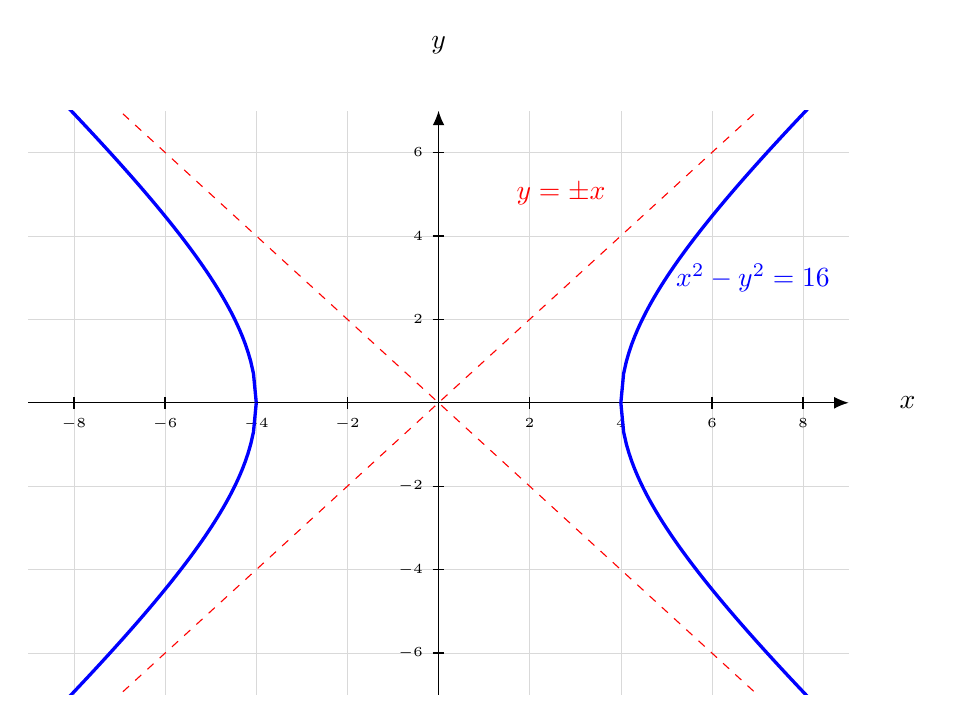
\begin{tikzpicture}
                    \begin{axis}[
                        axis lines=middle,
                        xlabel={$x$}, ylabel={$y$},
                        xlabel style={right},
                        ylabel style={above},
                        xmin=-9, xmax=9, ymin=-7, ymax=7,
                        xtick={-8,-6,-4,-2,0,2,4,6,8},
                        ytick={-6,-4,-2,0,2,4,6},
                        grid=both,
                        grid style={line width=.1pt, draw=gray!20},
                        major grid style={line width=.2pt,draw=gray!30},
                        samples=200,
                        domain=4:10,
                        restrict y to domain=-100:100,
                        width=12cm,height=9cm,
                        clip=true
                      ]

                      % Cabang kanan (y positif)
                      \addplot [very thick, blue, domain=4:10, samples=100] {sqrt(x^2 - 16)};
                      % Cabang kanan (y negatif)
                      \addplot [very thick, blue, domain=4:10, samples=100] {-sqrt(x^2 - 16)};
                      % Cabang kiri (y positive)
                      \addplot [very thick, blue, domain=-10:-4, samples=100] {sqrt(x^2 - 16)};
                      % Cabang kiri (y negative)
                      \addplot [very thick, blue, domain=-10:-4, samples=100] {-sqrt(x^2 - 16)};

                      % Asimtot y = x dan y = -x
                      \addplot [dashed, red, domain=-8:8] {x};
                      \addplot [dashed, red, domain=-8:8] {-x};

                      % Label hiperbola (opsional)
                      \node[blue,right] at (axis cs:5,3) {$x^2-y^2=16$};
                      \node[red,right] at (axis cs:1.5,5) {$y=\pm x$};
                    \end{axis}
                  \end{tikzpicture}
                \end{center}

          \item Pada bidang $xz$ (jika $y = 0$), maka diperoleh
                $
                  x^2 - z^2 = 16,
                $
                yaitu hiperbola terbuka ke arah sumbu $x$. Gambarnya seperti berikut.
                \begin{center}
                  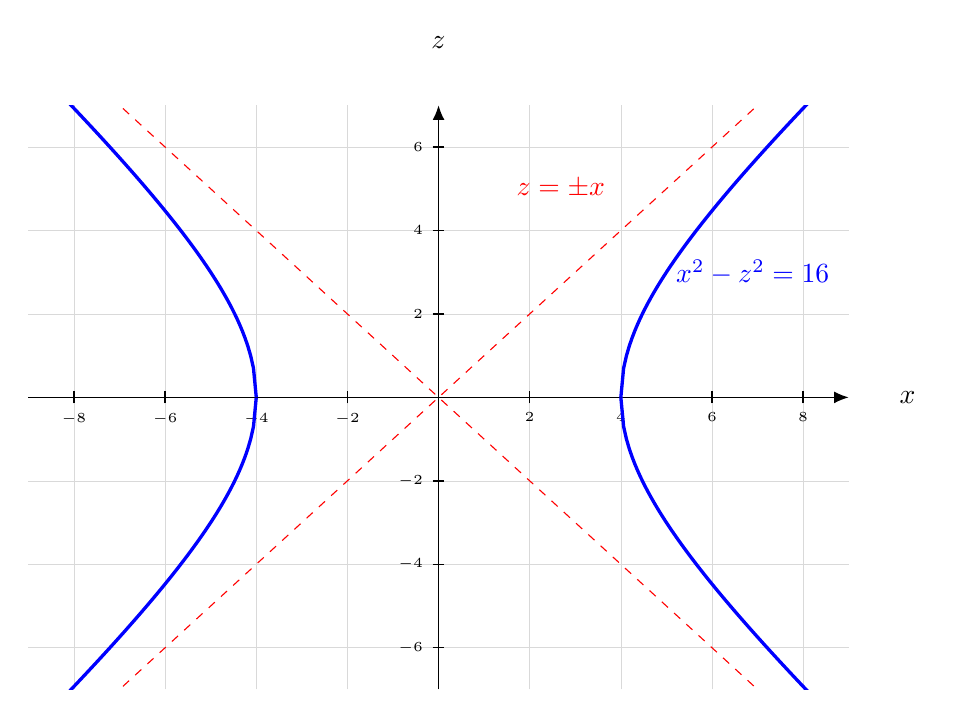
\begin{tikzpicture}
                    \begin{axis}[
                        axis lines=middle,
                        xlabel={$x$}, ylabel={$z$},
                        xlabel style={right},
                        ylabel style={above},
                        xmin=-9, xmax=9, ymin=-7, ymax=7,
                        xtick={-8,-6,-4,-2,0,2,4,6,8},
                        ytick={-6,-4,-2,0,2,4,6},
                        grid=both,
                        grid style={line width=.1pt, draw=gray!20},
                        major grid style={line width=.2pt,draw=gray!30},
                        samples=200,
                        domain=4:10,
                        restrict y to domain=-100:100,
                        width=12cm,height=9cm,
                        clip=true
                      ]

                      % Cabang kanan (z positif)
                      \addplot [very thick, blue, domain=4:10, samples=100] {sqrt(x^2 - 16)};
                      % Cabang kanan (z negatif)
                      \addplot [very thick, blue, domain=4:10, samples=100] {-sqrt(x^2 - 16)};
                      % Cabang kiri (z positive)
                      \addplot [very thick, blue, domain=-10:-4, samples=100] {sqrt(x^2 - 16)};
                      % Cabang kiri (z negative)
                      \addplot [very thick, blue, domain=-10:-4, samples=100] {-sqrt(x^2 - 16)};

                      % Asimtot z = x dan z = -x
                      \addplot [dashed, red, domain=-8:8] {x};
                      \addplot [dashed, red, domain=-8:8] {-x};

                      % Label hiperbola (opsional)
                      \node[blue,right] at (axis cs:5,3) {$x^2-z^2=16$};
                      \node[red,right] at (axis cs:1.5,5) {$z=\pm x$};
                    \end{axis}
                  \end{tikzpicture}
                \end{center}
          \item Pada bidang $yz$ (jika $x = 5$ atau $x = -5$), maka diperoleh
                $
                  -y^2 - z^2 = 16 - 25 = -9 \implies y^2 + z^2 = 9,
                $
                yaitu lingkaran dengan jari-jari $3$. Gambarnya seperti berikut.
                \begin{center}
                  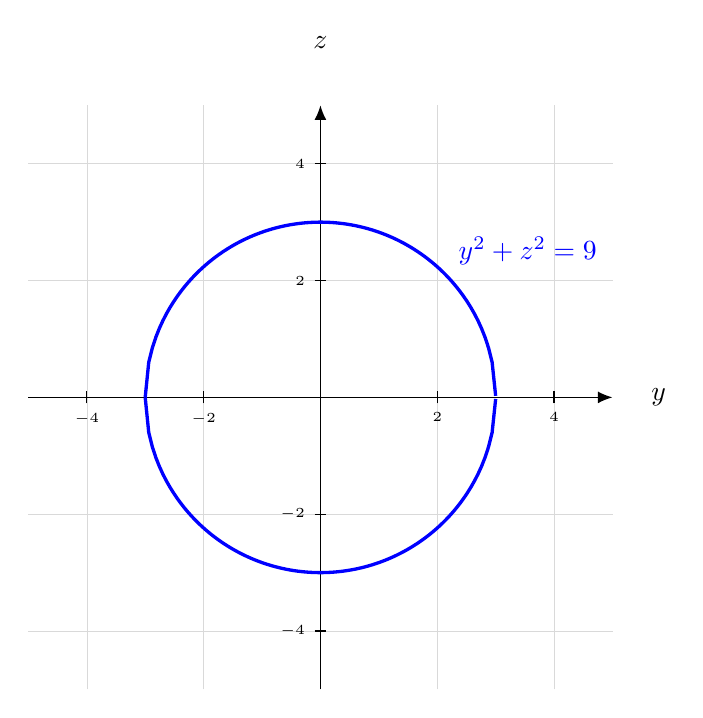
\begin{tikzpicture}
                    \begin{axis}[
                        axis lines=middle,
                        xlabel={$y$}, ylabel={$z$},
                        xlabel style={right},
                        ylabel style={above},
                        xmin=-5, xmax=5, ymin=-5, ymax=5,
                        xtick={-4,-2,0,2,4},
                        ytick={-4,-2,0,2,4},
                        grid=both,
                        grid style={line width=.1pt, draw=gray!20},
                        major grid style={line width=.2pt,draw=gray!30},
                        samples=200,
                        domain=-3:3,
                        restrict y to domain=-100:100,
                        width=9cm,height=9cm,
                        clip=true
                      ]

                      % Lingkaran y^2 + z^2 = 9
                      \addplot [very thick, blue, domain=-3:3, samples=100] {sqrt(9 - x^2)};
                      \addplot [very thick, blue, domain=-3:3, samples=100] {-sqrt(9 - x^2)};

                      % Label lingkaran (opsional)
                      \node[blue,right] at (axis cs:2.2,2.5) {$y^2+z^2=9$};
                    \end{axis}
                  \end{tikzpicture}
                \end{center}
        \end{itemize}
        Kemudian jika kita gabungkan ketiga gambar diatas dalam bentuk 3D, maka kita akan mendapatkan gambar berikut.
        \begin{center}
          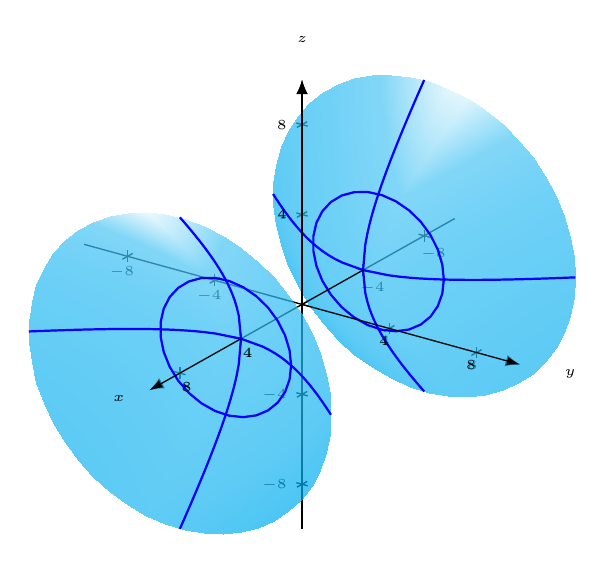
\begin{tikzpicture}
            \begin{axis}[
                legend pos=outer north east,
                axis lines = middle,
                xlabel style={left},
                ylabel style={right},
                zlabel style={above},
                xmin=-10, xmax=10,
                ymin=-10, ymax=10,
                zmin=-10, zmax=10,
                xtick={-8,-4,0,4,8},
                ytick={-8,-4,0,4,8},
                ztick={-8,-4,0,4,8},
                xticklabel style = {font=\tiny},
                yticklabel style = {font=\tiny},
                zticklabel style = {font=\tiny},
                xlabel = {\tiny $x$},
                ylabel = {\tiny $y$},
                zlabel = {\tiny $z$},
                legend style={cells={align=left}},
                legend cell align={left},
                view={125}{25},
                clip=false,
                point meta={z-abs(0.2*x+y)},
                unbounded coords=jump,
                width=11cm,height=11cm,
              ]
              % lower back part
              \addplot3[
                surf,
                shader=interp,
                opacity=0.7,
                samples=50,
                domain=4:8,
                y domain=0:360,
                variable=\u,
                variable y=\v,
              ]
              ({u}, {sqrt(u^2-16)*cos(v)}, {sqrt(u^2-16)*sin(v)});
              \addplot3[
                surf,
                shader=interp,
                opacity=0.7,
                samples=50,
                domain=-8:-4,
                y domain=0:360,
                variable=\u,
                variable y=\v,
              ]
              ({u}, {sqrt(u^2-16)*cos(v)}, {sqrt(u^2-16)*sin(v)});

              % x^2-z^2=16 di y=0
              \addplot3[thick,color=blue,samples y=1, domain=4:8, samples=30] (x, 0, {sqrt(x^2-16)});
              \addplot3[thick,color=blue,samples y=1, domain=4:8, samples=30] (x, 0, {-sqrt(x^2-16)});
              \addplot3[thick,color=blue,samples y=1, domain=-8:-4, samples=30] (x, 0, {sqrt(x^2-16)});
              \addplot3[thick,color=blue,samples y=1, domain=-8:-4, samples=30] (x, 0, {-sqrt(x^2-16)});

              % x^2-y^2=16 di z=0
              \addplot3[thick,color=blue,samples y=1, domain=4:8, samples=30] (x, {sqrt(x^2-16)}, 0);
              \addplot3[thick,color=blue,samples y=1, domain=4:8, samples=30] (x, {-sqrt(x^2-16)}, 0);
              \addplot3[thick,color=blue,samples y=1, domain=-8:-4, samples=30] (x, {sqrt(x^2-16)}, 0);
              \addplot3[thick,color=blue,samples y=1, domain=-8:-4, samples=30] (x, {-sqrt(x^2-16)}, 0);


              % y^2+z^2=9 di x=5
              \addplot3[thick, blue, domain=0:360, samples=30] (5, {3*cos(x)}, {3*sin(x)});
              % y^2+z^2=9 di x=-5
              \addplot3[thick, blue, domain=0:360, samples=30] (-5, {3*cos(x)}, {3*sin(x)});

              \draw[-{Latex[width=3pt]},black] (4,0,0) -- (10,0,0);
              \draw[-{Latex[width=3pt]},black] (0,0,0) -- (0,10,0);
              \draw[-{Latex[width=3pt]},black] (0,0,0) -- (0,0,10);
              \draw[black] (0,0,0) -- (-4,0,0);

              \node[anchor=east,, xshift=-2pt] at (axis cs:0,0,4) {{\tiny$4$}};
              \node[anchor=north, xshift=-2pt,yshift=0.5pt] at (axis cs:0,4,0) {{\tiny$4$}};
              \node[anchor=north, xshift=-2pt,yshift=0.5pt] at (axis cs:0,8,0) {{\tiny$8$}};
              \node[anchor=north, xshift=2.5pt] at (axis cs:4,0,0) {{\tiny$4$}};
              \node[anchor=north, xshift=2.5pt] at (axis cs:8,0,0) {{\tiny$8$}};
            \end{axis}
          \end{tikzpicture}
        \end{center}
  \item Diketahui $z^2=x^2 + y^2 - 4$ atau bisa kta tulis $z = \sqrt{x^2 + y^2 - 4}$. Agar lebih mudah, cukup kita turunkan secara implisit untuk persamaan $z^2=x^2 + y^2 - 4$.

        Ketika diturunkan secara implisit terhadap $x$, diperoleh
        \begin{align*}
          \frac{\partial}{\partial x}(z^2) & = \frac{\partial}{\partial x}(x^2 + y^2 - 4)  \\
          2z \frac{\partial z}{\partial x} & = 2x + 0 - 0                                  \\
          z_x                              & = \frac{x}{z}=\frac{x}{\sqrt{x^2 + y^2 - 4}}.
        \end{align*}
        Ketika diturunkan secara implisit terhadap $y$, diperoleh
        \begin{align*}
          \frac{\partial}{\partial y}(z^2) & = \frac{\partial}{\partial y}(x^2 + y^2 - 4)  \\
          2z \frac{\partial z}{\partial y} & = 0 + 2y - 0                                  \\
          z_y                              & = \frac{y}{z}=\frac{y}{\sqrt{x^2 + y^2 - 4}}.
        \end{align*}
        Kemudian, kita turunkan $z_x$ terhadap $x$ untuk mendapatkan $z_{xx}$.
        \begin{align*}
          z_{xx} & = \frac{\partial}{\partial x}\left(\frac{x}{z}\right)                            \\
                 & = \frac{z \cdot 1 - x \cdot z_x}{z^2}                                            \\
                 & = \frac{\sqrt{x^2 + y^2 - 4}  - x \frac{x}{\sqrt{x^2 + y^2 - 4}}}{x^2 + y^2 - 4} \\
                 & = \frac{(x^2 + y^2 - 4) - x^2}{(x^2 + y^2 - 4)^{3/2}}                            \\
                 & = \frac{y^2 - 4}{(x^2 + y^2 - 4)^{3/2}}
        \end{align*}
        Selanjutnya, kita turunkan $z_y$ terhadap $y$ untuk mendapatkan $z_{yy}$.
        \begin{align*}
          z_{yy} & = \frac{\partial}{\partial y}\left(\frac{y}{z}\right)                            \\
                 & = \frac{z \cdot 1 - y \cdot z_y}{z^2}                                            \\
                 & = \frac{\sqrt{x^2 + y^2 - 4}  - y \frac{y}{\sqrt{x^2 + y^2 - 4}}}{x^2 + y^2 - 4} \\
                 & = \frac{(x^2 + y^2 - 4) - y^2}{(x^2 + y^2 - 4)^{3/2}}                            \\
                 & = \frac{x^2 - 4}{(x^2 + y^2 - 4)^{3/2}}
        \end{align*}
        Terakhir, kita turunkan $z_x$ terhadap $y$ atau $z_y$ terhadap $x$ untuk mendapatkan $z_{xy}$.
        \begin{align*}
          z_{xy} & = \frac{\partial}{\partial y}\left(\frac{x}{z}\right)      \\
                 & = \frac{z \cdot 0 - x \cdot z_y}{z^2}                      \\
                 & = \frac{- x \frac{y}{\sqrt{x^2 + y^2 - 4}}}{x^2 + y^2 - 4} \\
                 & = \frac{-xy}{(x^2 + y^2 - 4)^{3/2}}
        \end{align*}

  \item Diketahui tinggi kerucut $h = 30\,\text{cm}$ dan jari-jari lingkaran alasnya $r = 10\,\text{cm}$. Kemudian diketahui pula kesalahan pengukuran tinggi kerucut $\Delta h = \pm 0.01h = \pm 0.3\,\text{cm}$ dan kesalahan pengukuran jari-jari lingkaran alasnya $\Delta r = \pm 0.005r = \pm 0.05\,\text{cm}$.
\end{enumerate}
\end{document}